\documentclass[../Paper.tex]{subfiles}
\usepackage{amsmath}
\usepackage{graphicx}
\usepackage{subfigure}
\usepackage{float}
\makeatletter % `@' now normal "letter"
\@addtoreset{equation}{section}
\makeatother  % `@' is restored as "non-letter"
\renewcommand\theequation{\oldstylenums{\thesection}%
                    .\oldstylenums{\arabic{equation}}}


\begin{document}
\section{Assumption and Theory}

\subsection{Hypothesis}

First of all, we propose the following three hypotheses, and all the following calculations and derivations are based on these three hypotheses:

(1)~The energy emitted by Sun during unit time is constant. 

(2)~The radiant energy absorbed by Mercury, Venus, and Earth is negligible;.

(3)~Only considered in the solar system. 

\subsection{List of Constants}

\renewcommand\arraystretch{1.5} % <-- 设置表格行高
\begin{table}[H]
\centering
\scriptsize %此处写字体大小控制命令
\begin{tabular}{p{2cm}<{\centering} p{6.5cm}<{\centering} p{3cm}<{\centering} %p{1cm}<{\centering} p{1cm}<{\centering} 
				p{1cm}<{\centering} p{1cm}<{\centering} }
		\hline
Symbol & Description & Value \\
	    \hline
	    \hline
$S.$ & Solar constant/W$\cdot s^{-2}$ & 1367 \\

$G$ & Universal gravitational constant/$m^3kg^{-1}s^{-2}$ & $6.67259\times10^{-11}$ \\

$R_E$ & The distance from the sun to the earth/m & $1.496\times10^{11}$ \\
		
$R_M$ & The distance from the sun to the Mars/m & $2.2794\times10^{11}$ \\

$M_S$ & The masse of the sun/kg & $1.9891\times10^{30}$  \\

$M_E$ & The masse of the earth/kg & $5.965\times10^{24}$  \\

$M_M$ & The masse of the Mars/kg & $6.4219\times10^{23}$  \\

$m$ & Total mass (sail plus payload)/kg & 2000~ \\

$T_E$ & The period of revolution of earth/s & $3.1536\times10^{7}$~(365days) \\

$T_M$ & The period of revolution of Mars/s & $5.93568\times10^{7}$~(687days)\\

$\omega_E$ & The angular velocity of revolution of earth/rad$\cdot s^{-1}$ & $1.9924\times10^{-7}$ \\

$\omega_M$ & The angular velocity of revolution of Mars/rad$\cdot s^{-1}$ & $1.0585\times10^{-7}$ \\
	    \hline
\end{tabular}

\caption{List of Constants}
\label{Table1}
\end{table}  

\subsection{Light pressure received by solar sail}

The solar constant (S.) refers to the solar radiation energy that received per second by per unit area of the top of the atmosphere circle perpendicular to the sunlight at the average distance from Sun to Earth ($D=1.496\times10^8km$). Similarly we denote S(r) as the energy flow density at the distance r from the Sun, and we denote $A$ as the area of solar sail.
\\

According to the conversation of energy:

\[S.\dfrac{4}{3}\pi{R_E}^2=S(r)\dfrac{4}{3}\pi r^2\]

\begin{equation}
S(r)=\dfrac{S.R_E^2}{r^2}
\end{equation}

The energy density is:\\
\begin{equation}
\rho_E=\dfrac{E}{V}=\dfrac{S.tAcos\alpha}{c tAcos\alpha}=\dfrac{S.}{c}
\end{equation}

The total light pressure is equal to twice of its energy density:
\begin{equation}
P(r)=2\rho_E=\dfrac{2S(r)}{c}=\dfrac{2S.{R_E}^2}{cr^2}
\end{equation}

The ideal plane solar sail model assumed that the impact of solar photon on the sail surface can be regarded as an ideal reflection, and the sail surface is an ideal plane. Therefore, the forces exert by incident photons and reflected photons are equal, shown as follows:

%-------------------这里插入射反射光的路径图---------------------%
\begin{figure}[H]
 \centering
 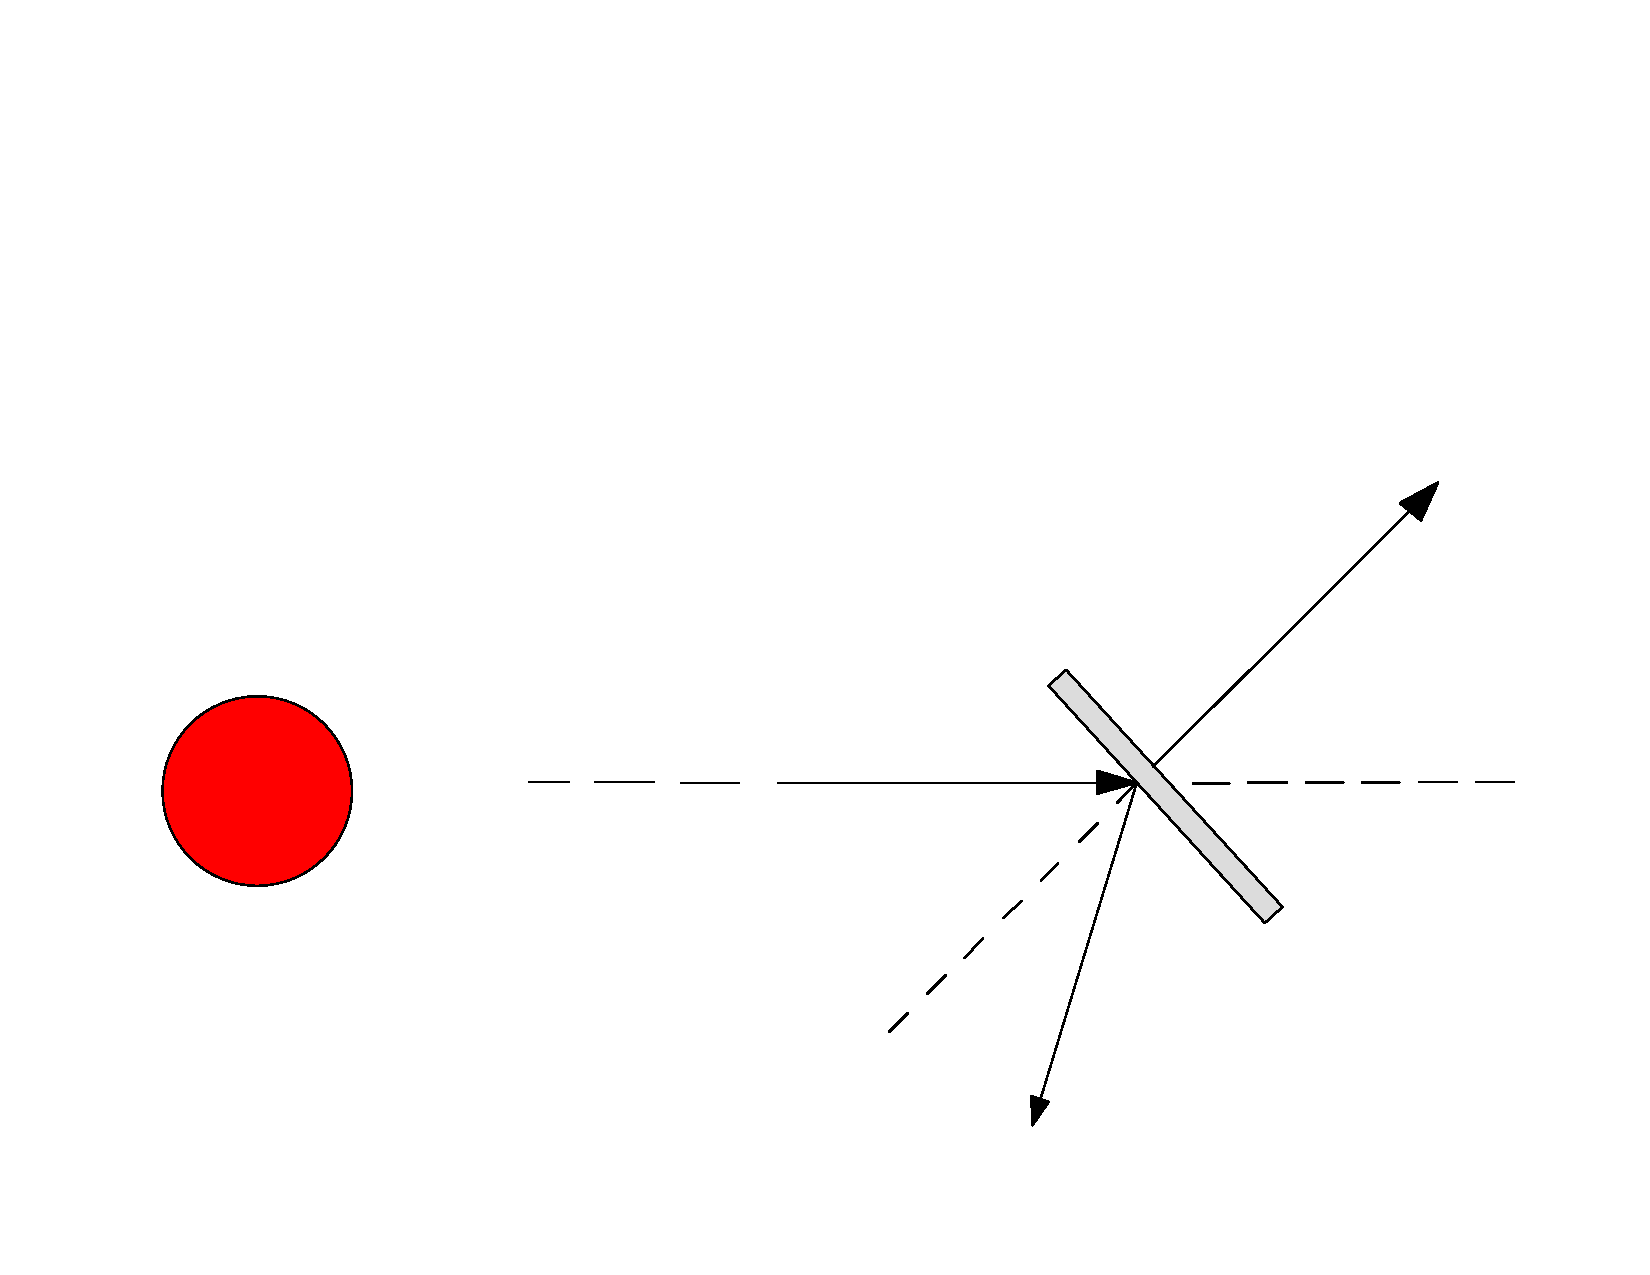
\includegraphics[scale=0.3]{../Figures/lightpressure.pdf}
 \caption{incident and reflected photon}
\end{figure}

The light pressure produced by the incident photon is:

\begin{equation}
P_i=\frac{P(r)}{2}A_z(cos\alpha~\vec{n}-sin\alpha~\vec{t})
\label{eq:1}
\end{equation}

In this formula, $A_z$ is the effective sail area, $\alpha$ is the angle between the incident ray and the solar sail unit normal direction $\vec{n}$, the unit vector of solar sail normal direction $\vec{n}$ is perpendicular to the sail plane and pointing out away from the sun. $\vec{t}$ is the tangent unit vector perpendicular to the normal $\vec{n}$, the anticlockwise direction is defined positive. Then the light pressure produced by the reflected light is as bellow:

\begin{equation}
P_r=\frac{P(r)}{2}A_z(cos\alpha~\vec{n}+sin\alpha~\vec{t})
\label{eq:2}
\end{equation}

The effective area refers to the area on which the sail is projected on the plane perpendicular to the sunlight, $A_z=Acos\alpha$. Therefore, the total light pressure acting on the ideal plane solar sail is:

\begin{equation}	
\vec{F_p}=\vec{F_i}+\vec{F_r}=P(r)Acos^2\alpha~\vec{n}=\dfrac{2S.{R_E}^2Acos^2\alpha}{cr^2}~\vec{n}
\label{eq:3}
\end{equation}

Therefore, the force of light pressure $F_p$ is always along the normal direction of solar sail surface, $\vec{f}=\vec{n}$, $\vec{f}$ is the unit vector of thrust, it is always in the direction along the pressure direction and deviates from the sun.

\subsection{Force analysis and acceleration}

In this problem, the solar sail is mainly affected by the gravity of Sun and the pressure of sunlight, because the magnitude of solar sail due to the gravitational action of Mercury, Venus and Earth is very small which can be neglected in comparing to the relative solar gravitation.

The solar sail is subjected to the small thrust from the continuous light pressure, and thrust itself is inversely proportional to the square of distance from Sun to the solar sail, so it can be realized with spiral trajectory.      

Light pressure is always deviated from the sun, by controling the attitude of solar sail, when the solar sail attitude angle $\alpha$ is positive, i.e. $F_p\cdot\alpha>0$, solar sail get orbital angular momentum, solar sail and spiral outward away from the sun; when the sail angle is negative, i.e. $F_p\cdot\alpha<0$, solar sail lose orbital angular momentum, and the solar sail moves toward the sun. 

\begin{figure}[H]
 \begin{minipage}[t]{0.5\linewidth}
 \centering{}
 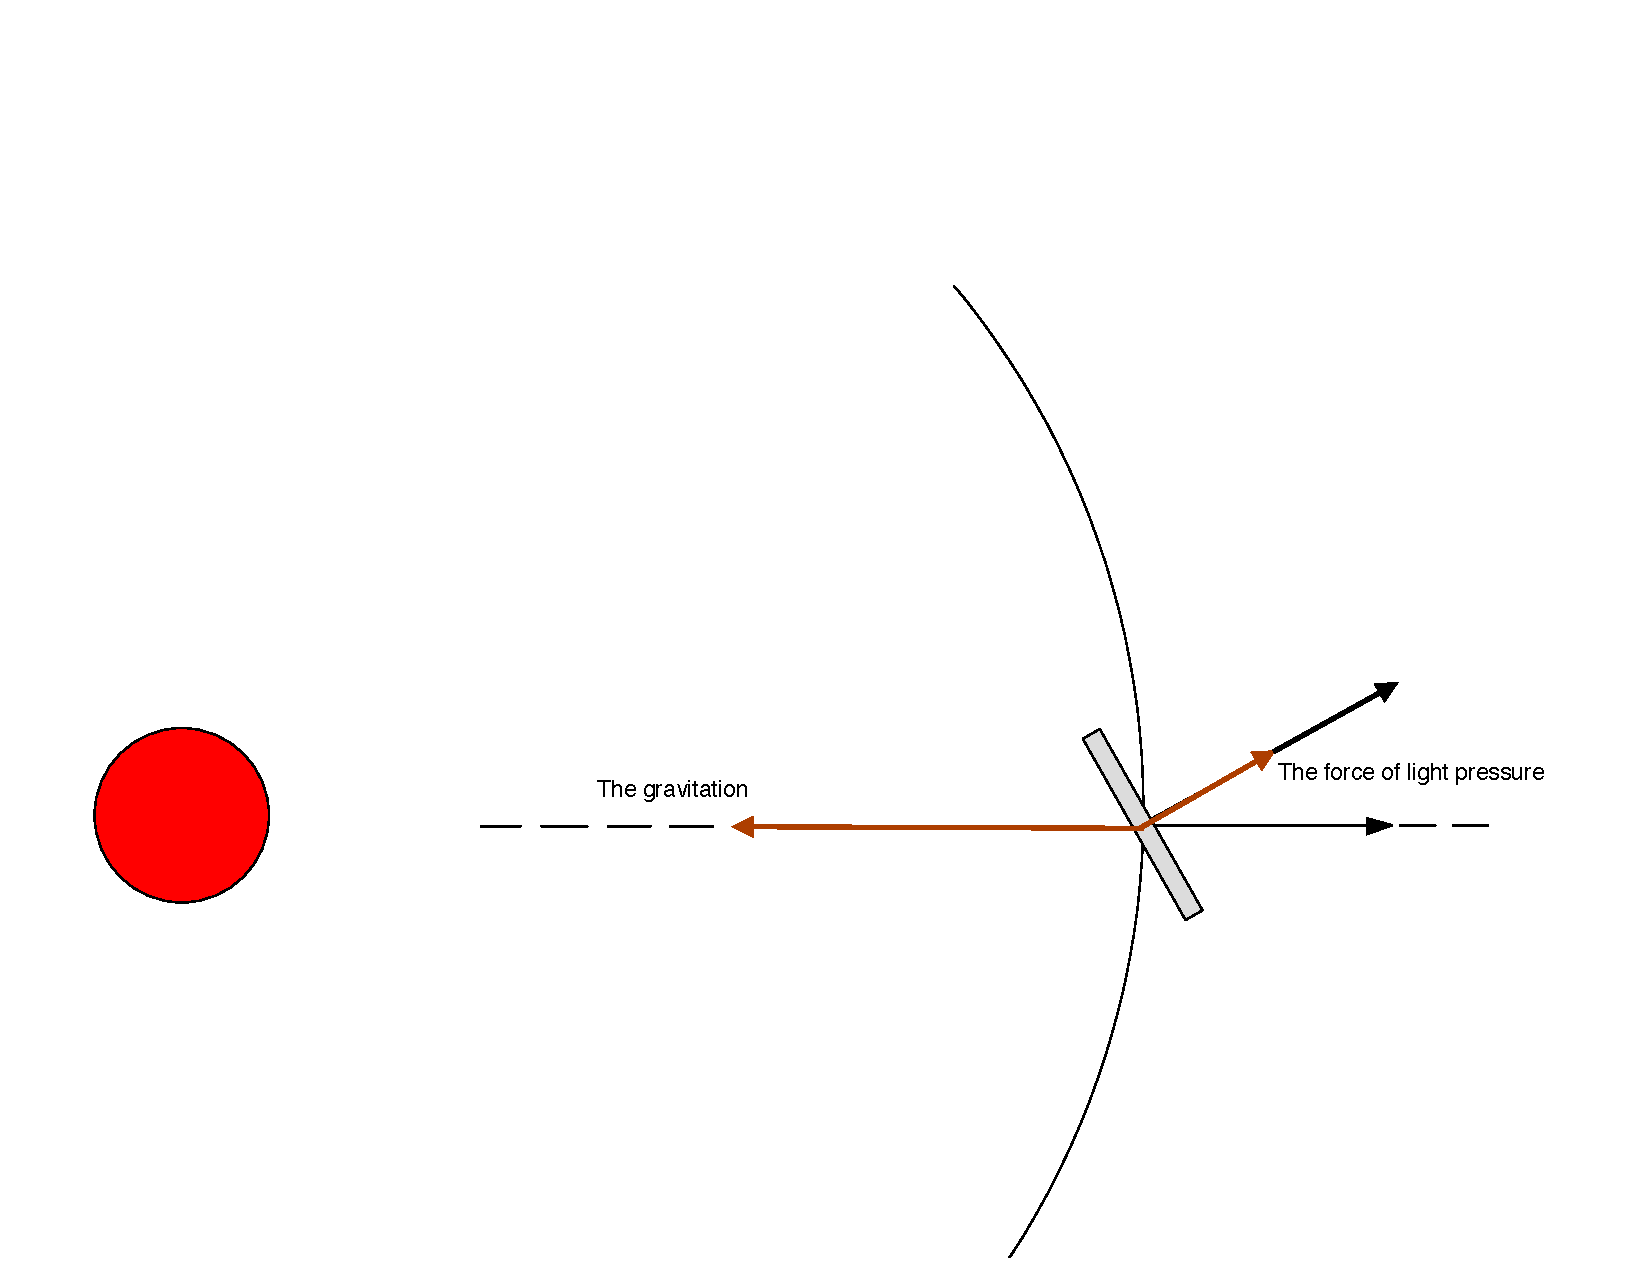
\includegraphics[width=2.2in]{accelerate.pdf}
 \caption{spiralling inward($F_P\cdot\alpha>0$)}
 \label{fig:side:a}
 \end{minipage}
 \begin{minipage}[t]{0.5\linewidth}
 \centering{}
 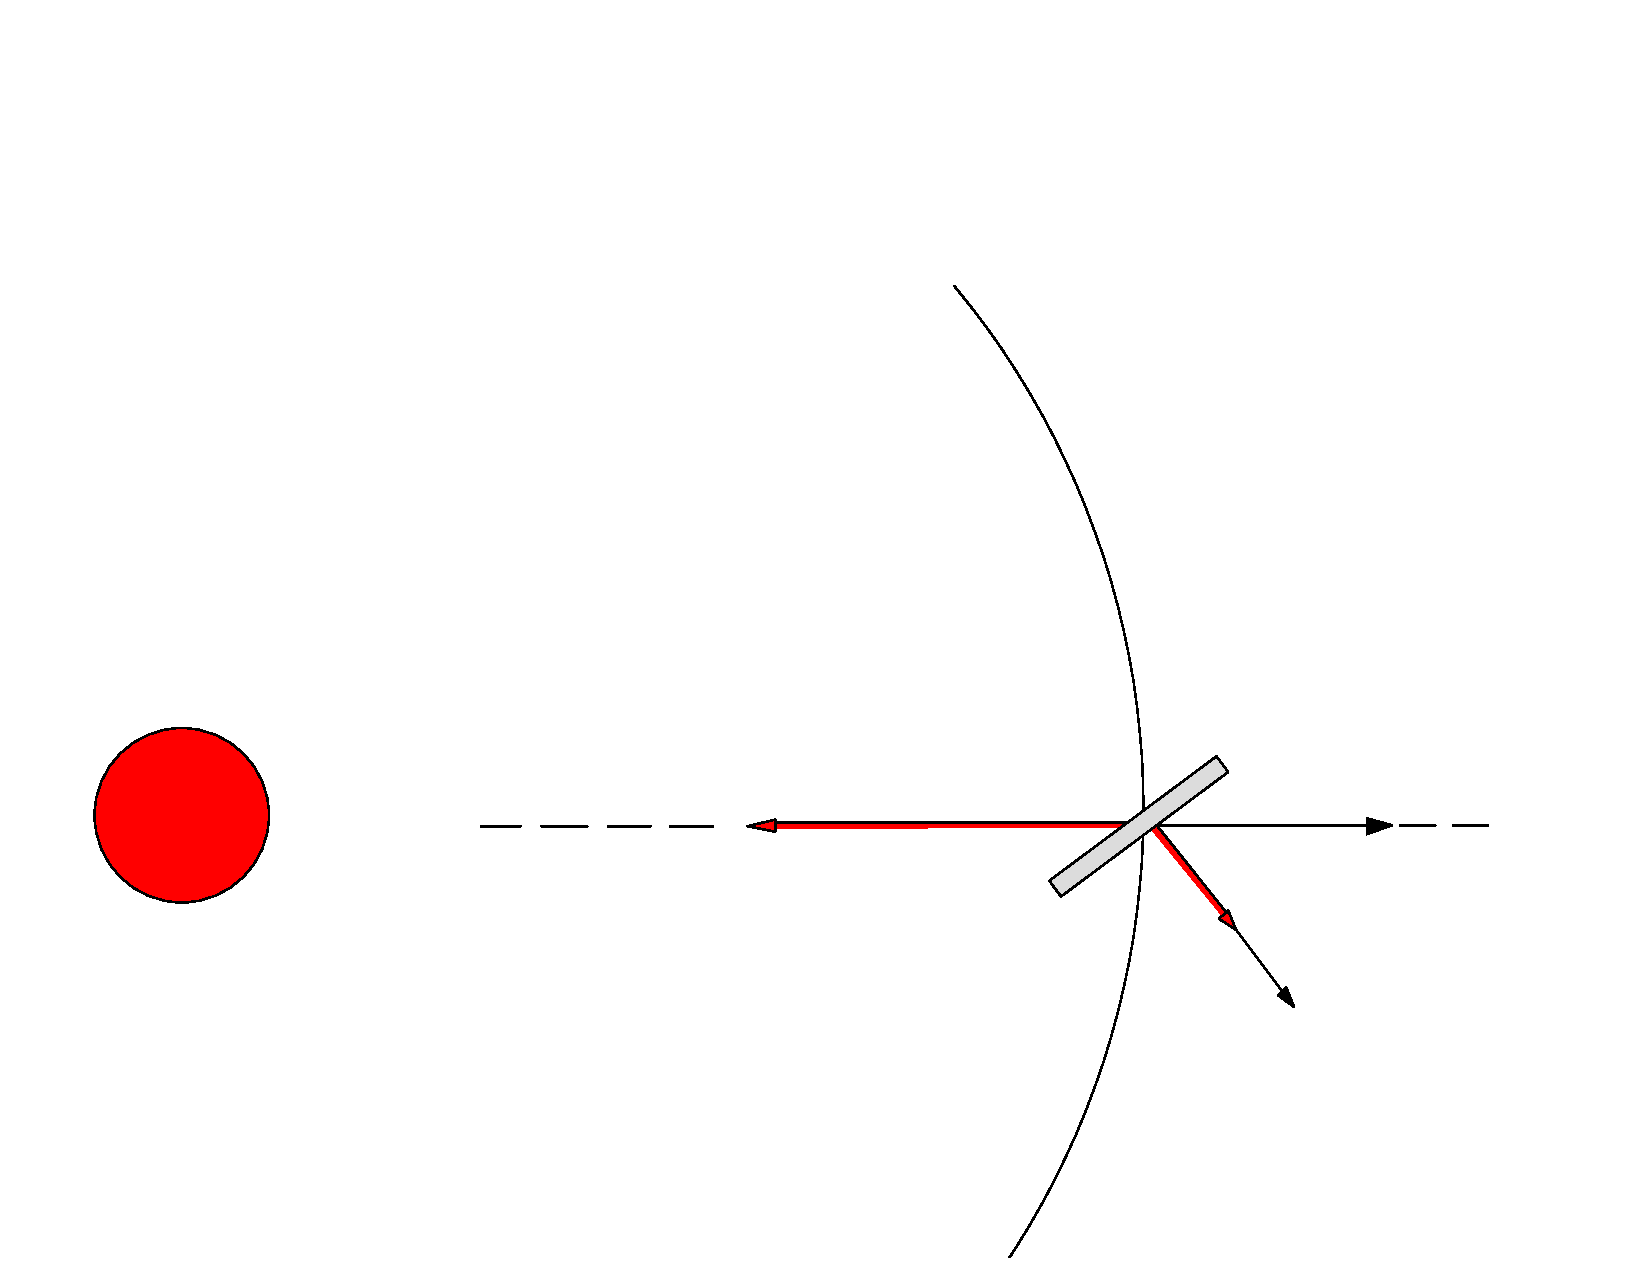
\includegraphics[width=2.2in]{../Figures/decrease.pdf}
 \caption{spiralling outward($F_P\cdot\alpha<0$)}
 \label{fig:side:b}
 \end{minipage}
\end{figure}

Denoted $F_g$ as the gravity of Sun received by solar sail and $F_g=G\dfrac{M_Sm}{r^2}$.

According to the Newton Second Law:

\begin{equation}
\vec{F_g}+\vec{F_p}=m\vec{a}
\end{equation}

projected to the radial direction:

\begin{equation}
G\dfrac{M_Sm}{r^2}+\dfrac{2S.{R_E}^2Acos^2\alpha}{cr^2}\cdot cos\alpha=ma
\end{equation}

so we obtain the normal acceleration as:

\begin{equation}
a=\dfrac{GM_S}{r^2}+\dfrac{2S.{R_E}^2Acos^3\alpha}{mcr^2}
\end{equation}

Numerical application:

\begin{equation}
a=\dfrac{13.27\times10^{19}}{r^2}+\dfrac{1.02\times10^{14}Acos^3\alpha}{r^2}
\end{equation}




\section{Basic Model}
\subsection{The initial state of the solar sail spacecraft}
First, considering the solar sail spacecraft will be launched from earth to Mars, and it needs to use the rocket to accelerate the spacecraft to earth's escape velocity. The best and most fuel-efficient situation here is that the energy that solar sails spacecraft is given by the rocket is just enough to get the spacecraft out of the earth's gravitational field, so, we are treating the speed of the solar sail with the speed of the earth's revolution speed  and direction.

\subsection{Theory}

\subsubsection{Assumptions of our model}

\subsubsection{Method}

\subsection{Model}
\subsubsection{model0}

\subsubsection{model1}

\begin{equation}
\vec{F_{flp}} = 2P(r)Acos^2(\alpha)\vec{n}
\end{equation}
and the gravitation from the Sun:
\begin{equation}
\vec{G}=-\frac{GMm}{r^2}\vec{u_r}
\end{equation}
We have the conversion relation between these vectors :
\begin{equation}
\vec{u_r}=cos\theta \vec{u_x} + sin\theta \vec{u_y}
\end{equation}
and
\begin{equation} 
\vec{u_\theta}=-sin\theta \vec{u_x} + cos\theta \vec{u_y}
\end{equation}
\begin{align*}
\vec{n} &= cos\alpha \vec{u_r} + sin\alpha \vec{u_\theta}\\
	    &= cos\alpha (cos\theta \vec{u_x} + sin\theta \vec{u_y}) + sin\alpha (-sin\theta \vec{u_x} + cos\theta \vec{u_y}) \\
	    &=(cos\alpha cos\theta - sin\alpha sin\theta )\vec{u_x} + (cos\alpha sin\theta + sin\alpha cos\theta)\vec{u_y}
\end{align*} 
Then we project this two force to the axe $x$ and axe $y$:
\begin{equation}
\vec{F_x} = (-\frac{GMmx}{(\sqrt{x^2+y^2})^3} + 2P(r)Acos^2\alpha(cos\alpha\frac{x}{\sqrt{x^2+y^2}} - sin\alpha\frac{y}{\sqrt{x^2+y^2}}))\vec{u_x}
\end{equation}



\end{document}